\chapter{Matheuristics}
On this chapter we will illustrate two heuristic solution for the TSP problem that are based on CPLEX.

\section{Hard fixing}
When we have to resolve a large instance of TSP, CPLEX can require a large amount of time. Moreover in some practical application we may have to resolve the problem in a certain amount of time that we cannot exceed. So for this reason we can set a time limit for CPLEX, that means that the solver will return the best solution found within that limit. The hard fixing algorithm starts from this point. Let's set a time limit (10 minutes for example) and consider the solution obtained. Of course this solution with high probability is not the optimum solution, but it may contains some edges that belong to it. So the idea is to fix some edges, and pass the new model to CPLEX. In order to do this we can simply work on the bounds of the variables: if we set $1 \leq x(i,j) \leq 1$ the corresponding edge is fixed on the solution. The new model of course is simpler, because we have a smaller amount of variables, so when we resolve it with CPLEX (again with a fixed time limit) it may find a better solution. This procedure can also be iterate until a final time limit (like 1 hour) is reached: each time we release the variables that were fixed on the previous iteration (just reset the bounds to $0 \leq x(i,j) \leq 1$) and we choose a new set of edges to fix.
Note that when the variables are fixed, due to the fact that the instance is smaller, CPLEX may resolve that model to its optimum before the time limit exceed.
Of course the choice of which edge to fix and their number is quite relevant. In general a good idea is to set a fixing percentage and randomly choose the variables to fix. We can also decide to variate the percentage over the iterations, for example starting with an high value (like 90\%) and then decrease it until zero. This mean that on the initial iterations the problem to resolve is very small so we may get a significant improve, while on the last iterations we have a big problem but lot of freedom to refine the solution. Of course this is only an example and other strategies can be implemented.  
\\\\ Our implementation of the Hard Fixing is presented in Algorithm \ref{alg:hf}. 
We used two variables to manage the time limit of the algorithm. The variable \textit{remaining\_time} keeps track of the time left to the algorithm to compute the solution. At beginning the variable assumes the value of the original time limit given by the user (line 2). The variable \textit{time\_x\_cycle} is the inner time limit and it is initially fixed to \textit{time\_limit/5} (line 3). Since with the inner time limit is very hard that an initial good solution will be computed, we provide to CPLEX a heuristic solution builded with the algorithm GRASP and refined with the 2-OPT algorithm (lines 4-6).
The algorithm then proceeds solving the problem within a while loop (line 7). At each iteration, we initially set the inner time limit as CPLEX environment parameter (lines 8 - 11). 
Then the solution, within the time limit, is computed (line 13) with the time needed to compute it (lines 12 and 14).
At this point, the variable \textit{remaining\_time} is updated subtracting from it the time taken by the solver (line 15).
\\ The variable \textit{percentage}, initially set to 90\% (line 1), is updated only if after two consecutive iterations the solution found doesn't improve of at least the 10\%. The update consists in subtracting 15\% from the previous percentage of fixed variables (line 18). Then the algorithm proceeds by resetting the lower bound of all variables to 0.0 (line 19), randomly selecting the indices of variables to be fixed and setting the lower bound of them to 1.0 (line 20). This sequence is repeated as long as the user-set time limit is reached.

\begin{algorithm}
    \caption{Hard Fixing}\label{Hard Fixing}
    
    \hspace*{\algorithmicindent} \textbf{Input:} $G = (V,E) , c : E \rightarrow \mathbb{R}$\\
    \hspace*{\algorithmicindent} \textbf{Output:} A solution for the TSP problem
    \begin{algorithmic}[1]
    \State $\textit{percentage} \gets \textit{0.9}$
    \State $\textit{remaining\_time} \gets \textit{timelimit}$
    \State $\textit{time\_x\_cycle} \gets \textit{timelimit / 5}$
    \State model $ \leftarrow $ \textbf{$\ast$ Initialize variables and objective function $\ast$ }
    \State first\_solution $ \leftarrow $ \textbf{$\ast$ Heuristic solution with GRASP + 2-OPT $\ast$ }
    \State model $ \leftarrow $  CPXaddmipstarts(first\_solution)
    \While {(\textit{remaining\_time} $>$ 0)} 
    	\If{$ (\textit{remaining\_time} > \textit{time\_x\_cycle})$} 
	\State $ model \gets $ CPX\_PARAM\_TILIM$(\textit{time\_x\_cycle}) $
	
	\Else \State $ model \gets $ CPX\_PARAM\_TILIM$(\textit{remaining\_time}) $
	\EndIf
	
	\State $\textit{t1} \gets \textit{second()}$
    	\State $\textbf{\textit{x}} \gets \text{solution}(\text{model}) $\;
	\State $\textit{t2} \gets \textit{second()}$
	\State $\textit{remaining\_time} \gets \textit{remaining\_time $-$ (t2 $-$ t1)}$
	\If{$ (\textit{remaining\_time} <= 0)$} 
	\State \textbf{break}
	\EndIf
	\State \textbf{$\ast$ If the solution doesn't improve (+10\%) twice in succession then $ percentage $ $ -$= $ 0.15. $ $\ast$}
	\State \textbf{$\ast$ Restore the default bounds for each variable $\ast$}
	\algstore{myalg}
    	\end{algorithmic}
	\label{alg:hf}
   	\end{algorithm}
	
	\begin{algorithm}                     
   	 \begin{algorithmic} [1]              
    	\algrestore{myalg}
	\State \textbf{$\ast$ Hard fixing of each variable according to \textit{percentage} $\ast$}
    \EndWhile
    \State \textbf{return} \textbf{\textit{x}} 
    \end{algorithmic}
    \end{algorithm}

\section{Local branching}
The strategy of this algorithm \cite{LB} is similar to the one of hard fixing: each iteration fix some edges in order to give to CPLEX a simpler version of the problem. However, rather then randomly choose the variable to fix, we let CPLEX decide which edges to maintain. We can achieve this with the introduction of a new constraint: let's consider an initial solution H provided by CPLEX within a time limit, let $x_e^H$ be the variables equals to one on this solution, we want the sum of these variables to be greater or equals than a percentage of the total number of edges. More formally:
\begin{equation*}
	\sum_{e \in E, \; x_e^H = 1} x_e \geq \alpha n
\end{equation*}
where $\alpha$ is the selected percentage and n is the size of the instance. In other word with this constraint we are telling CPLEX that we want a percentage of variables that are in the initial solution to be also in the final solution. At this point we can give the new model to CPLEX that will resolve it within the time limit, automatically deciding which variables to maintain.
Of course this is not a valid constraint for the problem, cause we are not sure that the variables equals to one on a solution belong to the optimum.\\
Again we can iterate the procedure, each time removing the old constrain and generating a new one, based on the new solution, until a final time limit is reached. The fact that the selection of the variables to fix is not random, means that the CPLEX solution is deterministic, so it is not wise to execute two iterations with the same fixing percentage, cause we may resolve two times the same problem obtaining the same solution within the time limit.
Finally, another shrewdness that is required, is that this algorithm works only if the fixing percentage is very high, so iteration with percentage of 50-60 or less should be avoided. 
\\\\ Our implementation of the Local branching is presented in Algorithm \ref{alg:lb}. The implementation is pretty similar to Algorithm \ref{alg:hf}, for this reason we only emphasise the differences between the two algorithms. 
At each iteration of the while loop (line 7), the variables of the solution are saved and a new local branching constraint is added to the model, removing the previous one. The known term of the constraint, that is the variable \textit{percentage} in the algorithm, is initially set to: number of nodes $\ast$ 0.95 (line 1) and is updated with the same conditions as Algorithm \ref{alg:hf}, but in this case subtracting from the variable \textit{percentage} the value: number of nodes $\ast$ 0.05 (lines 18 - 21). As in algorithm \ref{alg:hf}, the sequence is repeated as long as the user-set time limit is reached.

\begin{algorithm} [H]
    \caption{Local branching}\label{Local branching}
    \hspace*{\algorithmicindent} \textbf{Input:} $G = (V,E) , c : E \rightarrow \mathbb{R}$\\
    \hspace*{\algorithmicindent} \textbf{Output:}  A solution for the TSP problem
    \begin{algorithmic}[1]
    \State $\textit{percentage} \gets \textit{$|$V $|$ $\ast$ $0.95$}$
    \State $\textit{remaining\_time} \gets \textit{timelimit}$
    \State $\textit{time\_x\_cycle} \gets \textit{timelimit / 5}$
    \State model $ \leftarrow $ \textbf{$\ast$ Initialize variables and objective function $\ast$ }
    \State first\_solution $ \leftarrow $ \textbf{$\ast$ Heuristic solution with GRASP + 2-OPT $\ast$ }
    \State model $ \leftarrow $  CPXaddmipstarts(first\_solution)
    \While {(\textit{remaining\_time} $>$ 0)} 
    	\If{$ (\textit{remaining\_time} > \textit{time\_x\_cycle})$} 
	\State $ model \gets $ CPX\_PARAM\_TILIM$(\textit{time\_x\_cycle}) $
	
	\Else \State $ model \gets $ CPX\_PARAM\_TILIM$(\textit{remaining\_time}) $
	\EndIf
	\State $\textit{t1} \gets \textit{second()}$
    	\State $\textbf{\textit{x}} \gets \text{optimal\_solution}(\text{model}) $\;
	\State $\textit{t2} \gets \textit{second()}$
	\State $\textit{remaining\_time} \gets \textit{remaining\_time $-$ (t2 $-$ t1)}$
	\If{$ (\textit{remaining\_time} <= 0)$} 
	\State \textbf{break}
	\EndIf
	\State \textbf{$\ast$ If the solution doesn't improve (+10\%) twice in succession then $ percentage $ $ -$= $ (0.05 \ast percentage).$ $\ast$}
	\State \textbf{$\ast$ Save the indices of the solution variables. $\ast$}
	\State \textbf{$\ast$ If is not the first cycle remove the last row of the model. $\ast$}
	\State \textbf{$\ast$ Add the new local branching constraint with $\alpha n = percentage. $ $\ast$}
    \EndWhile
    \State \textbf{return} \textbf{\textit{x}}
    \end{algorithmic}
    \label{alg:lb}
    \end{algorithm}

\section{Final comparison between Matheuristics}
The instances used to compare heuristic algorithms are the following: 

\begin{multicols}{3}
    \begin{itemize}
        \item d657.tsp
        \item d1291.tsp
        \item fl417.tsp
        \item fl1400.tsp
        \item fl1577.tsp
        \item nrw1379.tsp
        \item p654.tsp
        \item pcb1173.tsp
        \item pcb3038.tsp
        \item pr1002.tsp
        \item pr2392.tsp
        \item rl1304.tsp
        \item rl1323.tsp 
        \item rl1889.tsp
        \item u724.tsp
        \item u1060.tsp
        \item u2152.tsp
        \item u2319.tsp
        \item vm1084.tsp
        \item vm1748.tsp
    \end{itemize}
    \end{multicols}
    
\noindent
For each problem $i$ and algorithm $j$, we compare the Gap computed as
\begin{equation}
	gap_{ij} \; (\%) = { objFunc_j(i) - objFunc_{opt}(i) \over objFunc_j(i) } * 100,
\end{equation}
\noindent
where $objFunc_j(i)$ is the objective function value computed by the algorithm $j$ for the problem $i$.
The method used to compute a solution within the time limits is the \textit{Generic Heuristic Callback}, which is the best exact algorithm we implemented (see Section \ref{callbackresults}). The time limit has been set to 30 minutes.
In figure \ref{fig:Math} you can see the performance profile of the Matheuristic algorithms. The Hard Fixing outperforms the Local Branching in most of instances. Even if worse, the Local Branching algorithm achieves a gap within twice the best, so it is considered by us a valid competitor. 
From our experiments we observed that Matheuristics achieve the optimum in several instances, even in a problem with 2319 nodes. We also noticed that Matheuristic algorithms work very well even with big instances, achieving an objective function value within 5\% from optimum. All the numerical results are reported in Section \ref{resultMath}.  
The reason for their good performance may be due to the powerful \textit{Generic Heuristic Callback} algorithm which, thanks to Concorde, generates numerous cuts on fractional solutions, and also provides heuristic solutions to the solver thanks to a quick and effective algorithm (see Section \ref{callHeu}). Another reason is that our Matheuristic algorithms exploit all time available by fixing a decreasing number of variables.

\begin{figure}[H]
\centering
	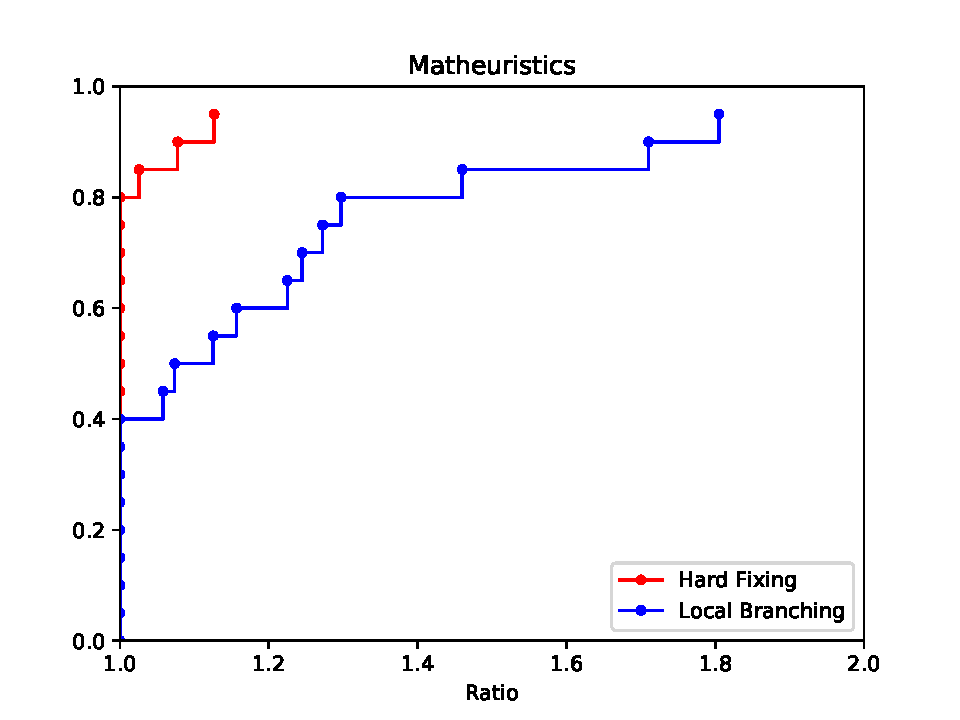
\includegraphics[scale=0.9]{media/Math.pdf} \\
	\caption{Performance profile of Matheuristics}
	\label{fig:Math}
\end{figure}
